% GENERAL REMARKS / COMMENTS
	% Dette er 'THE MAIN Master Document'.
	% Den skal ha en fin forside, god struktur, og \include{} alle kapitlene etterhvert som de skrives.
	% Husk målene som står i karaktersettingen når du ser på strukturen og oppbygningen. Det skal være ryddig og originalt, og en god skriftlig presentasjon.

	% Inspirasjons-maler:
		% (M1) i Overleaf: "UiO, Department of Informatics: Master's Thesis Template 2020"
		% (M2) i Overleaf: "UiO Master Thesis"
		% Gode eksemplel-thesis'er
			% E.g. Tønnes Nygaard sin
	% Følger foreløpig (M1) (foruten alle \usepackage'r og \titleformat'er).








% DECLARATIONS & INITIALIZATIONS / PREAMBLE
	% DEFINING DOCUMENT CLASS
	\documentclass[a4paper, english]{article}

	% USING PACKAGES
	\usepackage[utf8]{inputenc}
\usepackage{csquotes}
\usepackage[backend=biber,sortcites]{biblatex}
\usepackage{Assets/DUO/duomasterforside}
\usepackage[dvipsnames]{xcolor} % for å kunne et større nummer fargemodeller i en mer fleksibel pakke
\usepackage{amsmath} % for equation*-environmentet
\usepackage{subcaption} % for subfigure-environmentet


% Considering to use:
	% \usepackage[big]{titlesec} % to customize chapters, sections, and sub-sections style in an easy way — https://www.overleaf.com/learn/latex/Sections_and_chapters
	% \usepackage{sectsty} % to customize sections, sub-sections, paragraphs, and sub-paragraphs

% Previously looked at but not found useful yet:
	% \usepackage{sidecap} % for juxtapositioning minipages next to each-other horizontally
	% \usepackage{scalerel} % for scaling objects according to references

	% SETTING NEW COMMANDS AND FUNCTIONS
	% Text-editing
\newcommand{\tit}[1]{\textit{#1}}
\newcommand{\tbf}[1]{\textbf{#1}}

% Colors
\newcommand{\tcol}[2][red]{\textcolor{#1}{#2}} % default-color is red

% Page-Spacing, -Margins, and -Padding
\newcommand{\nl}{\newline}
\newcommand{\np}{\newpage}

% Lists
\newcommand{\subdash}[1]{\begin{itemize} \item{#1} \end{itemize}}

	% ADDING BIBLIOGRAPHY REFERENCE-DATABASE
	\addbibresource{Assets/Bibliography/reference_database.bib}







% BODY
\begin{document}
% HEADER
	\title{Computational Self-Awareness in Musical Robotic Systems} % med eller uten \\ før "in"
	% \subtitle{\tcol{Endowing musical robots with self-awareness — }An experimental study}	INKLUDER?
	\author{David Thorvaldsen}
	\duoforside[dept={Institute for Informatics}, program={Informatics: Robotics and Intelligent Systems}, long]

	\pagenumbering{roman}
	\section*{Abstract}
	\newpage

	\section*{Acknowledgements}
	\newpage

	\tableofcontents
	\newpage

	\listoftables
	\newpage

	\listoffigures
	\newpage

	\pagenumbering{arabic}
	\setcounter{page}{1}








% MAIN (ALL THE SECTIONS INPUT)
	% INTRODUCTION, CHAPTER 1
	\chapter{Introduction}
	% Here's where my journey begins. I have Lucas Paruch and Viktoria Stray's wish of "good and best of luck!" (except that I don't believe in luck)
	
	
	
	
	
	
	
	
	% CONSIDER HOW MUCH OF THIS BELONGS HERE, AND WHAT BELONGS IN THE Abstract.
	% Subsection 1.1
	\section{Motivation}
	
	Grunnene til å studere effektene av selv-bevissthet.
	\nl
	
	De viktigste bidragene av MSc thesis-arbeidet summert \tcol[gray]{(for å få det til å stå frem/ut bedre enn å bare "gjemme" det i den siste delen av oppgaven)}.
	
	
	
	
	
	
	
	
	
	% Subsection 1.2
	\section{Goal of the thesis}
	% Research Goals / Goal of the thesis:
	\besk{"to make the reader better understand what the thesis is about"—Jim, og "en rød tråd?"—Sigmund}
	
	Spesifikke mål \tcol[gray]{(goals/aims)} med master-oppgaven/-prosjektet. Hva jeg vil vise/demonstrere til folk \tcol[gray]{(leserne f.eks.)} om self-awareness \tcol[gray]{(SA)} og hvordan.
	\nl
	
	\textbf{Research Question 1}:
	
	Will performance in collective multi-robot systems increase as the level of Self-Awareness increases? Specifically, will increased levels of Self-Awareness in the individual agents/musical robots lead to the collective of individuals being able to synchronize to each other faster than with lower levels of Self-Awareness? \nl
	
	\textbf{Research Question 2}:
	
	Will increased levels of Self-Awareness lead to more robustness and flexibility in terms of handling environmental noise and other uncertainties — specifically in the continued ability of musical robots to synchronize to each other efficiently despite these difficulties/challenges? \nl
	
	
	
	
	
	
	
	% Subsection 1.3
	\section{Outline}
	En fin \tcol[gray]{(Eagle's-eye)} oversikt over strukturen til hele dette dokumentet fra nå av, og utover.


	% BACKGROUND, CHAPTER 2
	\chapter{Background}
% SE PÅ SamuelsenS MASTEROPPGAVE FOR INSPIRASJON (TROR HAN CLUSTERA OG KLASSIFISERTE HOVEDKONSEPTENE HAN BYGDE PÅ).
Kulepunkter \tcol[gray]{(bulletpoints)} fra mulige inspirasjoner og referanser \tcol[gray]{(pga. "Write a few lines summarizing relevant articles one comes across (which one is likely to refer to in the final report)" — Jims master-skrivingsdokument)}.



% SECTION 1

\section{Taking inspiration from natural phenomena}
The intriguing, diverse, and complex phenomena of nature have for long served as exciting inspirations to human engineers and researchers [ant-colonies, boids, swarms, beeclust]. One other such phenomena, studied and modelled, is the synchronously firing fireflies in forests, as can be seen an example of in Figure \ref{fig:synched_fireflies_phenomenon}.

\begin{figure}[!ht]
	\centering
	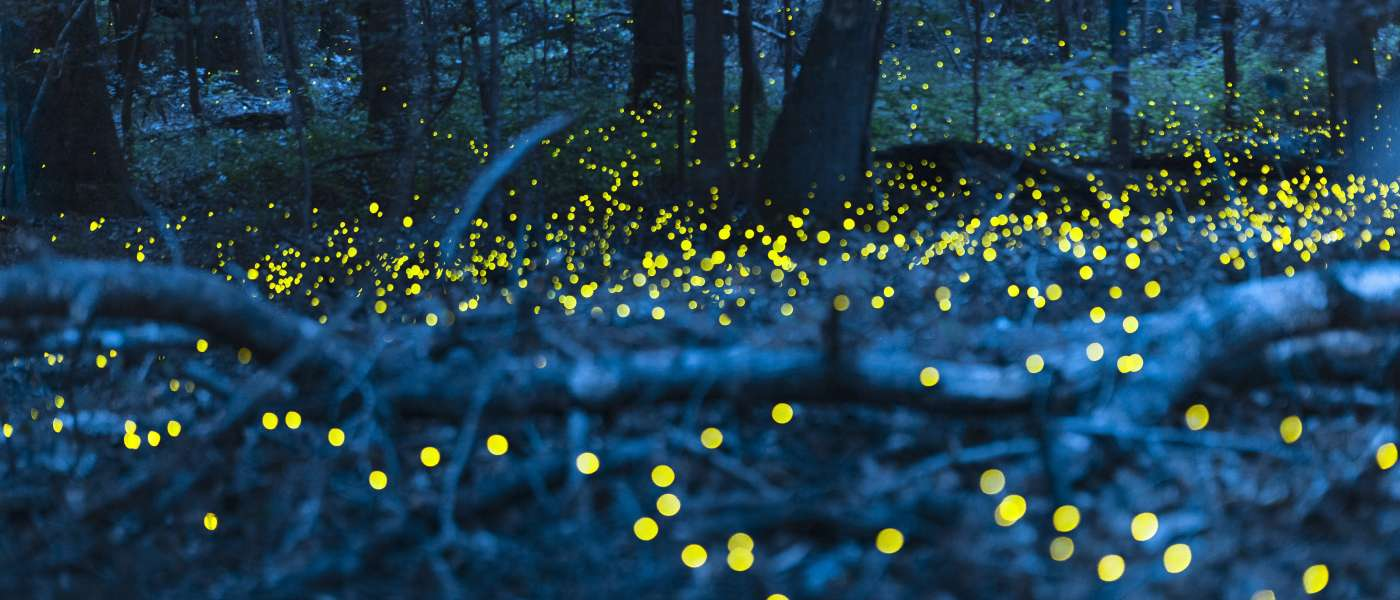
\includegraphics[width=0.9\linewidth]{Assets/Figures/synchronized_fireflies_phenomenon.jpg}
	\caption{Synchronous fireflies at Congaree National Park, United States \cite{synched_fireflies_phenomenon}.}
	\label{fig:synched_fireflies_phenomenon}
\end{figure}

This phenomenon of fireflies synchronizing to each other has inspired scientists like Mirollo \& Strogatz \cite{mirollo_strogatz_PCO_synch} and in later time Kristian Nymoen et al. \cite{nymoen_synch}, to model and replicate this natural phenomenon in human-engineered systems. It turns out that this is not a biological, but mathematical, problem. Given the periodic and repeating nature of the flashing/firing of the fireflies, modelling a firefly has been done by looking at each firefly as a periodic signal or oscillator. This work \cite{mirollo_strogatz_PCO_synch, nymoen_synch} then ties into the broader work on synchronizing oscillators which has been subject to study for some time now []. What separates Mirollo-Strogatz and K. Nymoen's approaches from these other and previous oscillator-synchronizing methods, is mainly that here the oscillators are \textit{pulse-coupled} (which the fireflies also can be said to be), as opposed to the more ``standard'' and constraining \textit{phase-coupled} oscillators.






% SECTION 2

\section{Oscillators and oscillator-synchronization}

	\gjor{Beskriv dette så godt at du kan snakke fritt om oscillatorers \textbf{faser} og \textbf{frekvenser} senere (i Implementation f.eks.), spesielt i tilfelle for noen ikke har vært borti det før, eller tatt et Signalbehandlings-kurs}
	
	\gjor{Skill på Pulse-coupled Oscillators, og Phase-coupled Oscillators}
	
	Much of the terminology from \cite{nymoen_synch} is used here. An oscillator $i$ is characterized by its \textit{phase} $\phi_i(t)$, which is—at the start of its periodic signal period—initialized to 0 and evolves towards 1 at a rate of $\frac{d \phi_i(t)}{d t}$ — which is also called the \textit{frequency} of the oscillator. When oscillator $i$'s phase is equal to 1 (i.e. when $\phi_i(t)=1$, or when the periodic signal period is over), we say oscillator $i$ has \textit{phase-climaxed}.
	
	\subsection{Phase-adjustment}
				
	(If relevant and wanted) \nl
	Previous approaches to Phase-synchronization in oscillators (pulse- and/or phase-coupled).
		
	\subsection{Frequency-adjustment}
	
	(If relevant and wanted) \nl
	Previous approaches to Frequency-synchronization in oscillators (pulse- and/or phase-coupled) [fixed\_freqs, fixed\_range\_freqs] where the oscillators's frequencies are either equal and fixed, or where frequencies are bound to initialize and stay within a fixed interval/range.
	
	% TOOLS & ENGINEERING ?
	\section{\question{Tools and engineering}}
	\describe{(Hentet fra Tønnes sin master) En introduksjon til de forskjellige verktøyene og prosessene brukt iløpet av masteroppgaven. Fokuser på fysisk arbeid gjort, og ingeniør-delene av masteroppgaven, inkludert 3D-design av de fysiske robotene, valg av deler, simulering i systemer, og testingen, valideringen, og verifikasjonsmetoder brukt i oppgaven. Gjerne også en oversikts-tabell av verktøy og programvare brukt}
	
	
	% PROPOSED ALGORITHM ?
	\section{\inkl{Proposed Algorithm?}}
	\besk{Metoden/Ideen bak mitt bidrag/forslag, forklart i detalj}

	
	% BENCHMARK ?
	\section*{Benchmark?}
	DET SAMME SOM SEKSJONEN 'Implementation'?
	\nl
	
	PRESENTERING AV METODEN BRUKT TIL Å EVALUERE PERFORMANCEN AV DEN FORESLÅTTE/PROPOSED'E ALGORITMEN. FØRST ER KANSKJE EN REFERANSE-ALGORITME BRUKT FOR SAMMENLIKNING BESKREVET. DERETTER ER (F.EKS. OBJEKTIV-) FUNKSJONER BRUKT I TESTENE FORKLART. ENDELIG (TIL SLUTT) ER KANSKJE MILJØENE (ENVIRONMENTS'A) OG PARAMETERNE BRUKT PRESENTERT.

	% IMPLEMENTATION (METHOD-EQUIVALENT)
	\chapter{Implementation}
\besk{Her presenterer jeg re-implementasjonen/etterlikningen/implementasjonsspesifikke-valg av K. Nymoens approach og teori i det nye systemet/simulatoren min i Unity — samt hvordan jeg har verifisert at mekanismene fungerer (e.g. fase-synkroniseringsplott)}

% Introducing the Chapter to what I've done/developed
This chapter gives an overview of the developed musical multi-robot system, methods implemented for it, as well as the performance measure used to evaluate these methods. The main goal of the implemented system is to allow for individual musical agents in a musical multi-agent collective to interact with each other, in order to achieve emergent and co-ordinating behaviour—in our case synchronization—with varying degrees of self-awareness, collective-sizes, and of difficulty and certainty in the environment and communication. More specifically, the goal with the design is to enable the robot collective to achieve so-called \textit{harmonic synchronization} within a relatively short time. Exactly what is meant by \textit{harmonic synchronization} will be expounded in Section \ref{sec:harmonic_synchrony}.

These goals firstly require of the agents the modelling of oscillators with their properties, like phase and frequency, as explained further in Subsection \ref{subsec:agent}. To allow for interaction and communication between the agents, mechanisms so that the agents can transmit "fire"-signals, as well as listen for other agents's "fire"-signals, is necessary as well, and is presented in Subsection \ref{subsec:fire_signal}.

First, the system and the system components will be presented and introduced. Then, methods implemented for achieving the system target goal of \textit{harmonic synchrony} in various synchronization objectives—firstly solely for oscillator-phases, then secondly for both oscillator-phases and oscillator-frequencies—will be described and presented. How the system target state of harmonic synchrony is detected will then be described in Section \ref{sec:performance_measure}.




% SECTION 1, Introducing my System and its System-components:
\section{Simulator setup: the musical multi-robot collective}
\label{sec:developed_system}
	\besk{Introduserer og presenterer det utviklede (simulator-)systemet du har utviklet i Unity selv}

	Envision that we have a decentralized (i.e. no central control) multi-agent collective scenario consisting of musical robots modelled as oscillators. These are solely communicating through brief ``fire''-like audio-signals—greatly inspired by K. Nymoen et al.'s synchronizing ``fireflies'' \cite{nymoen_synch}. They are not initially synchronized in their firing of audio-signals; but as time goes, they are entraining to synchronize to each other by adjusting their phases and frequencies when/after hearing each other's audio-/fire-signals. If they then, after some time of listening to each other and adjusting themselves accordingly, succeed in becoming synchronized — we then will eventually see ``fire''-events/-signals line up at an even underlying pulse or rhythm. Examples and demonstrations of this process are depicted in Figure \ref{fig:first_idea:first_fig} and Figure \ref{fig:first_idea:second_fig}.

	% First Intro-illustration figure to easily get a quick idea of what the system/design does/consists of (to be exchanged with a describing system scheme/diagram):
	\begin{figure}[h]
	\centering
	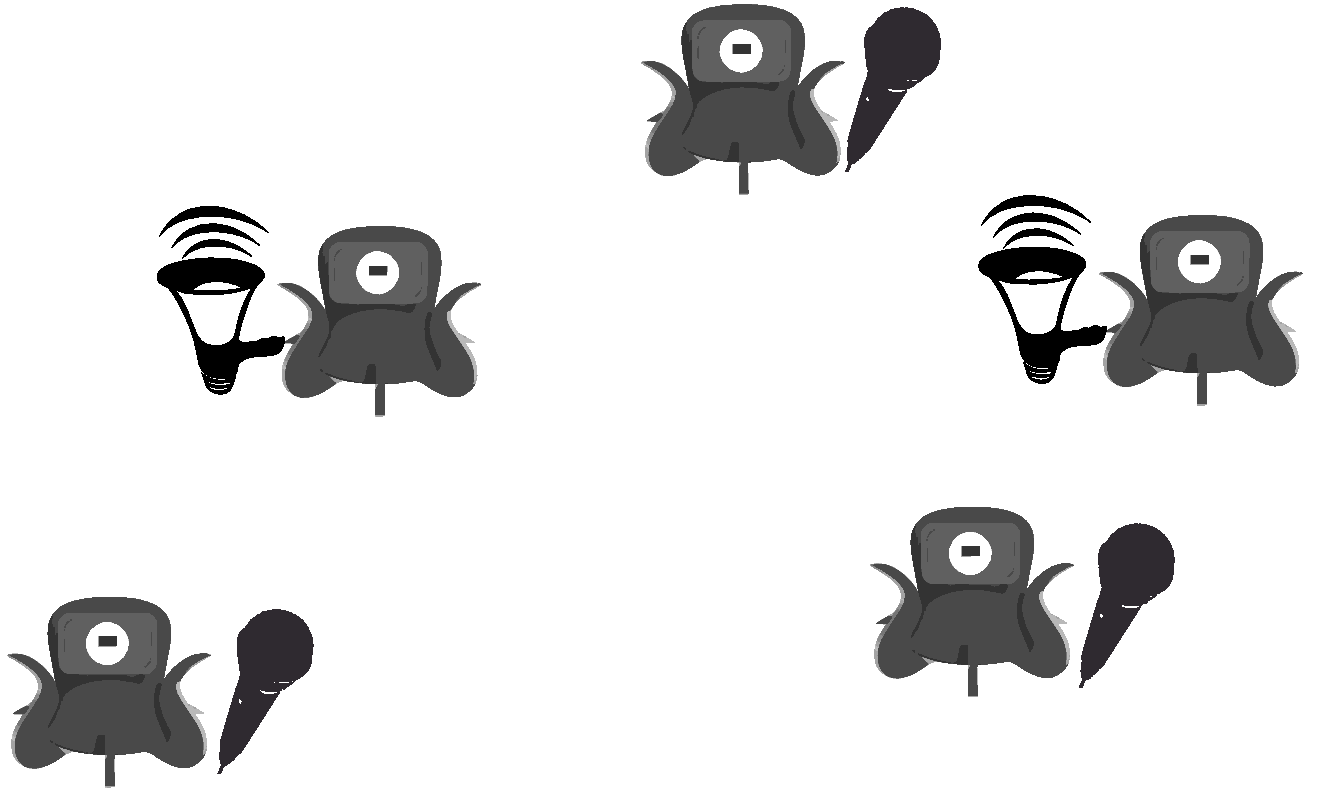
\includegraphics[width=0.9\linewidth]{Assets/Figures/schematic_initial_idea.pdf}
	\caption[Illustration/schematic of the developed multi musical robot collective/system]{Illustration/Schematic: The musical robot collective entraining to synchronize to each other, or more specifically to achieve harmonic synchronization, through performing phase- \& frequency-adjustments. Agents that are not firing at the moment will adjust themselves after hearing a transmitted ``fire''-/adjustment-signal from a neighbouring firing agent.}
	\label{fig:first_idea:first_fig}
	\end{figure}

	% Second Intro-illustration figure to easily get a quick idea of what the system/design does/consists of (to be exchanged with a describing system scheme/diagram):
	\begin{figure}[ht!]
		\centering
			\begin{subfigure}[t]{.5\textwidth}
				\centering\captionsetup{width=.9\linewidth}%
				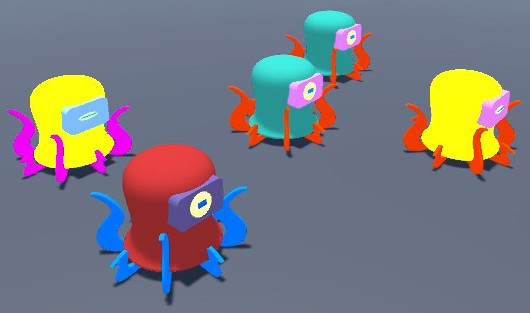
\includegraphics[width=0.9\linewidth]{Assets/Figures/squiggles_unsynched_in_simulation.jpg}
				\caption{Screenshot from the very beginning of a Synchronization-simulation.}
				\label{fig:first_idea:second_fig:unsynched}
			\end{subfigure}%
			\begin{subfigure}[t]{.5\textwidth}
				\centering\captionsetup{width=.9\linewidth}%
				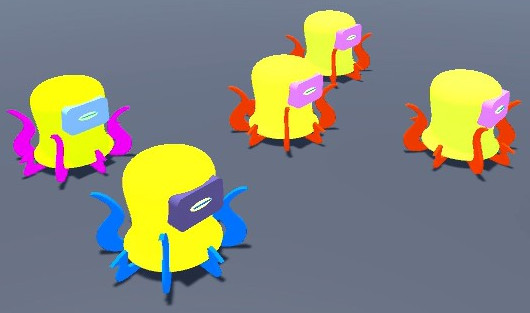
\includegraphics[width=0.9\linewidth]{Assets/Figures/squiggles_synched_in_simulation.jpg}
				\caption{Screenshot from the same Synchronization-simulation as in \ref{fig:first_idea:second_fig:unsynched}, a few moments later.}
				\label{fig:first_idea:second_fig:synched}
			\end{subfigure}
		\caption[Synchronization-example/-screenshots from simulation in Unity]{From simulation: An example of the system target goal of harmonic synchrony being achieved in a musical robot collective, where oscillator-frequencies $\omega$ are constant and equal (1Hz), or in other words synchronized already, but oscillator-phases $\phi$ are unsynchronized and initially uniformly random numbers in the range of $[0,1]$. \nl
		At first in \ref{fig:first_idea:second_fig:unsynched}, we see the agents firing, i.e. blinking with their eyes and turning their body yellow, asynchronously at first. Only two robots, one with pink and one with red tentacles, fire synchronously so far. Seconds later, after having listened to each others's adjustment-signals and adjusted themselves accordingly, all agents now fire simultaneously and synchronously, as can be seen in \ref{fig:first_idea:second_fig:synched}.}
		\label{fig:first_idea:second_fig}
	\end{figure}

	% \inkl{Noe om hyperparameterne?}

	% INCLUDE PHASES UNSYNCHED VS. SYNCHED PLOT? See 'Relevant MSc-thesis Concerns'.
		% % Phase-/time-plot Figure with two Subplots. Subplot 1: phase-/time-plot when oscillators are unsynchronized. Subplot 2: phase-/time-plot when oscillators are synchronized
		% \begin{figure}[h]
			% \centering
				% \begin{subfigure}[t]{.5\textwidth}
					% \centering\captionsetup{width=.9\linewidth}%
					% 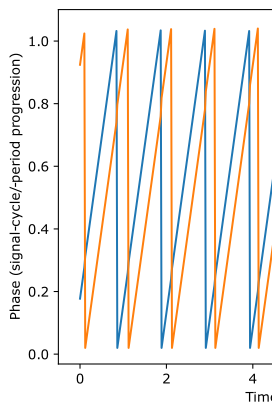
\includegraphics[width=0.9\linewidth]{Assets/Figures/phases_unsynched.png}
					% \caption{Oscillators are initially not (phase-) synchronized.}
					% \label{fig:phases_unsynched}
				% \end{subfigure}%
				% \begin{subfigure}[t]{.5\textwidth}
					% \centering\captionsetup{width=.9\linewidth}%
					% 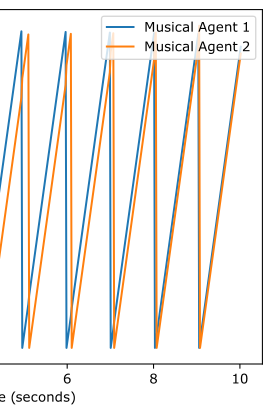
\includegraphics[width=0.9\linewidth]{Assets/Figures/phases_synched.png}
					% \caption{Oscillators are now, seconds later, (phase-) synchronized.}
					% \label{fig:phases_synched}
				% \end{subfigure}
			% \caption{Phase-plots for the agents}
			% \label{fig:initial}
		% \end{figure}




	% Introducing my own System Components:
	
	% Om den enkelte noden/agenten min med alle egenskaper den har osv.
	\subsection{The individual agent: a musical robot}
	\label{subsec:agent}
		As introduced and presented earlier, our musical robot collective will then consist of models of M. J. Krzyzaniak and RITMO's \textit{Dr. Squiggles}, 3D-models of which can be seen in Figure \ref{fig:first_idea:second_fig}.
	
		Every musical robot or node have certain components, attributes, and characteristics that make it what it is. Such include an oscillator-component, consisting of the agent's oscillator-phase $\phi$ and oscillator-frequency $\omega$. Notions like ``agent'', ``robot'', ``firefly'', and ``oscillator'' will be used interchangeably throughout the thesis. The agents have an input-mechanism for hearing/detecting transmitted ``fire''-event signals from other agents, as well as an output-mechanism for transmitting or playing such ``fire''-/adjust-signals or tones, as is illustrated with the microphone and megaphone respectively in Figure \ref{fig:first_idea:first_fig}.
		
		In order to be able to analyse the musical scenario within which they are situated (self-assessment), as well as for adapting their musical output accordingly (self-adaptation), the agents are to some extent endowed with artificial intelligence and self-awareness capabilities. The robots are self-aware of their own phase and frequency, but are unaware of other agents's true phases and frequencies. They also possess the self-assessment capability of evaluating how much in- or out-of-synch they are, as seen in the greater context of the entire robot collective. When the agents hear the transmitted ``fire''-/adjust-signals, the agents are intelligent enough to adjust themselves in the direction of the system goal/target state.

		



	% Om kommunikasjonen til agentene mine: audio-/``fire''-signalet
	\subsection{Robot communication: the ``fire''-signal}
	\label{subsec:fire_signal}
	
	These aforementioned audio-signals, also referred to as ``fire''-signals, ``flash''-signals, or adjust-signals, are transmitted whenever an agent's oscillator \textit{peaks} or \textit{climaxes} (i.e. after its cycle or period is finished, having phase $\phi(t)=1$) — or actually after every second \textit{peak}, as a way (discovered by K. Nymoen et al. \cite{nymoen_synch}) to attain the system target goal of \textit{harmonic synchrony}, to be elaborated upon in Section \ref{sec:harmonic_synchrony}.

	The ``fire''-signals are short and impulsive tones that the agents output through their loudspeakers. These short audio-signals/sounds ``wildly'' transmitted or played into the environment are then the only means of communication within the multi-agent collective, implying that are agents are pulse-coupled, not phase-coupled, oscillators. In other words, our agents will communicate and co-ordinate with each other through the very typical multi-agent system concept of \textit{stigmergy}.
	
	When an agent detects a ``fire''-/adjust-signal, the agent will adjust its own oscillator-properties (phase $\phi$ and frequency $\omega$), depending on which type of problem the agents are to solve. No individual agent is directly able to adjust or modify the state or properties of any other agent, only its own. Exactly the type of problems we attempt to solve in this thesis will be presented now in Section \ref{sec:phase_methods} and Section \ref{sec:frequency_methods}.
	
	
	
	
	
	
	
	
	




% SECTION 2, Presenting new Methods I implemented myself for Phase-Adjustment:
\section{Synchronizing oscillator-phases}
\label{sec:phase_methods}
	\gjor{Introduser det første $\phi$-problemet, uthevet og i fet skrift. Deretter fortsett til løsningene dens (Phase-Adj.-metodene). "This is the first and simpler problem to solve, namely synchronizing the phases $\phi_i$ of all agents $i$."}

	If we first assume constant and equal oscillator-frequencies in our agents, we can take a look at how the agents adjust their|initially random|phases in order to synchronize to each other. We will from here on and out refer to this first problem as \textbf{the $\phi$-problem}, given that the phases ($\phi_i$) for all agents $i$ are what we need to adjust and synchronize — and that frequencies ($\omega_i$) technically already are synchronized.
	
	The goal state of the agents is now for all agents to fire/flash simultaneously, after having started firing/flashing at random initially. Note that this is a special case of the final and ultimate goal of \textit{harmonic synchrony}. This is due to how all agents in the collective firing/flashing simultaneously, is considered having achieved harmonic synchrony since its phases would be synchronized if fire-events are lined up in even pulses, as well as all frequencies in the agent collective being within the set of ``legal'' frequencies, $\omega_{0} \cdot 2^{\mathbb{N}_0}$, where $\omega_0$ is the fundamental (smallest) frequency in the agent collective, and $0 \in \mathbb{N}_0$ — leading to $\omega_0 \cdot 2^0 = \omega_0$ to be a legal frequency, which is what all agents in our case here have as frequences.
	
	In order for the musical agents to synchronize to each other, they will have to—due to their heterogenous and randomly initialized phases—adjust or update their own phases according to some well-designed update-/adjustment-functions, as presented below.
	
	When it comes to the temporality and timing of when these updating functions are used and applied; Musical agents's phases get updated/adjusted immediately as ``fire''-/``flash''-events from neighbouring robots are perceived.
	
	
	
	% Mirollo-Strogatz's Phase-Adjustment
	\subsection{Mirollo-Strogatz's ``standard'' phase-adjustment} % used '-adjustment' before
	
	Mirollo-Strogatz's approach for synchronizing phases in oscillators, as introduced in \ref{mirollo_strogatz_phase_adjust}, is implemented in the Unity simulator, and each agent is endowed with \textbf{phase update function \eqref{strog_phase}} with which they adjust themselves according to when perceiving a ``fire''-signal as described above.
	
	The verification that this works in the newly built synchronization-simulator was performed by dumping all agents's phase-values $\phi(t)$ during simulation-runs. A plot of these $\phi(t)$-values, evolving through simulation-time in seconds, is shown in Figure \ref{fig:strog_phase}.
	
	\begin{figure}[h]
		\centering
		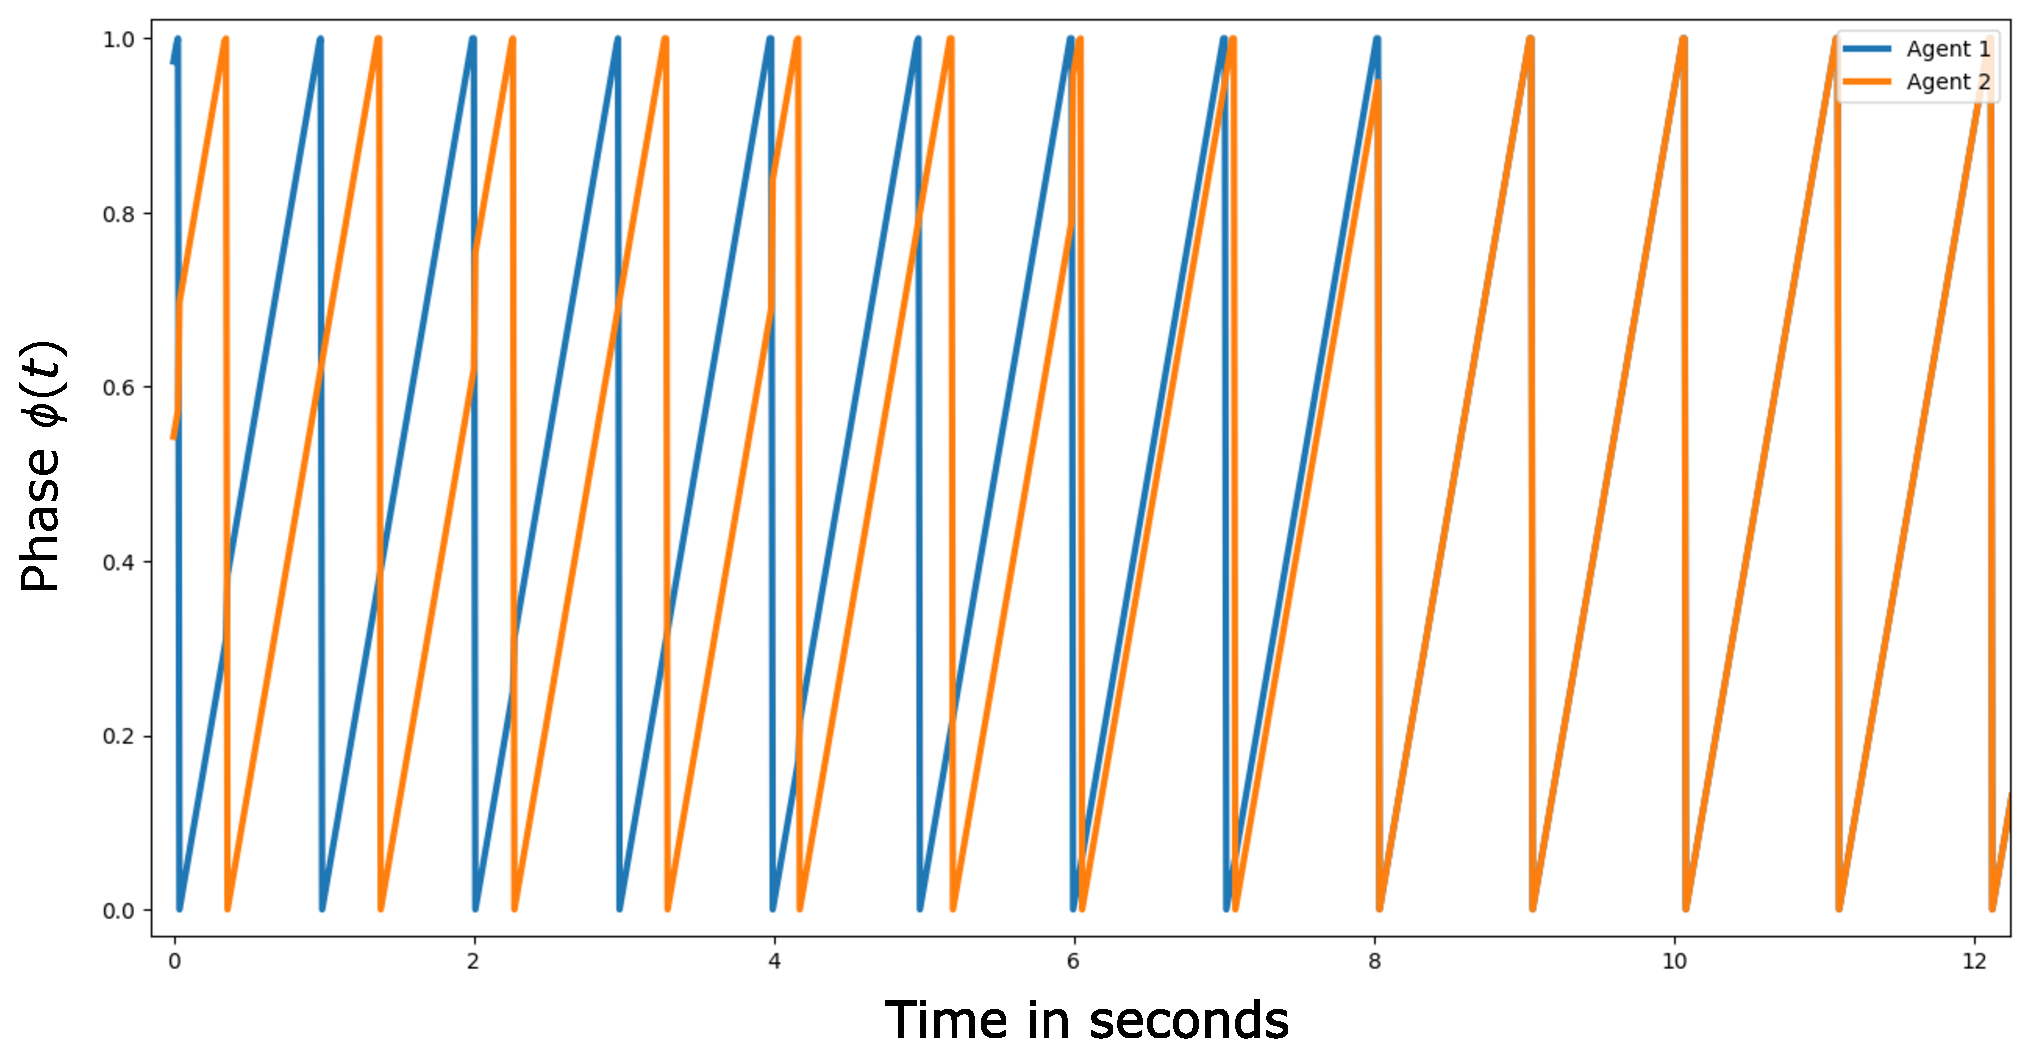
\includegraphics[width=0.9\linewidth]{Assets/Figures/MirolloStrogatzPhaseAdjustmentSecondTry.pdf}
		\caption[Illustration of Mirollo-Strogatz's ``standard'' phase-adjustment]{``Standard'' phase-adjustment with Mirollo-Strogatz's approach}
		\label{fig:strog_phase}
	\end{figure}
	
	
	
	
	% K. Nymoen's bi-directional phase-adjustment
	\subsection{K. Nymoen's bi-directional phase-adjustment} % used 'Shifts' before
	
	K. Nymoen et al.'s approach for synchronizing phases in oscillators, as introduced in Section \ref{nymoen_phase_adjust}, is implemented in Unity, and each agent is endowed with \textbf{phase update function \eqref{nymoen_phase}} with which they adjust themselves according to when perceiving a ``fire''-event as described above.
	
	The verification that this works in the newly set-up simulator-environment was performed by analysing carefully all the agents's phase-values $\phi(t)$ throughout a simulation-run. Such an analysis/plot can be seen in Figure \ref{fig:nymoen_phase}.
	
	\begin{figure}[h]
		\centering
		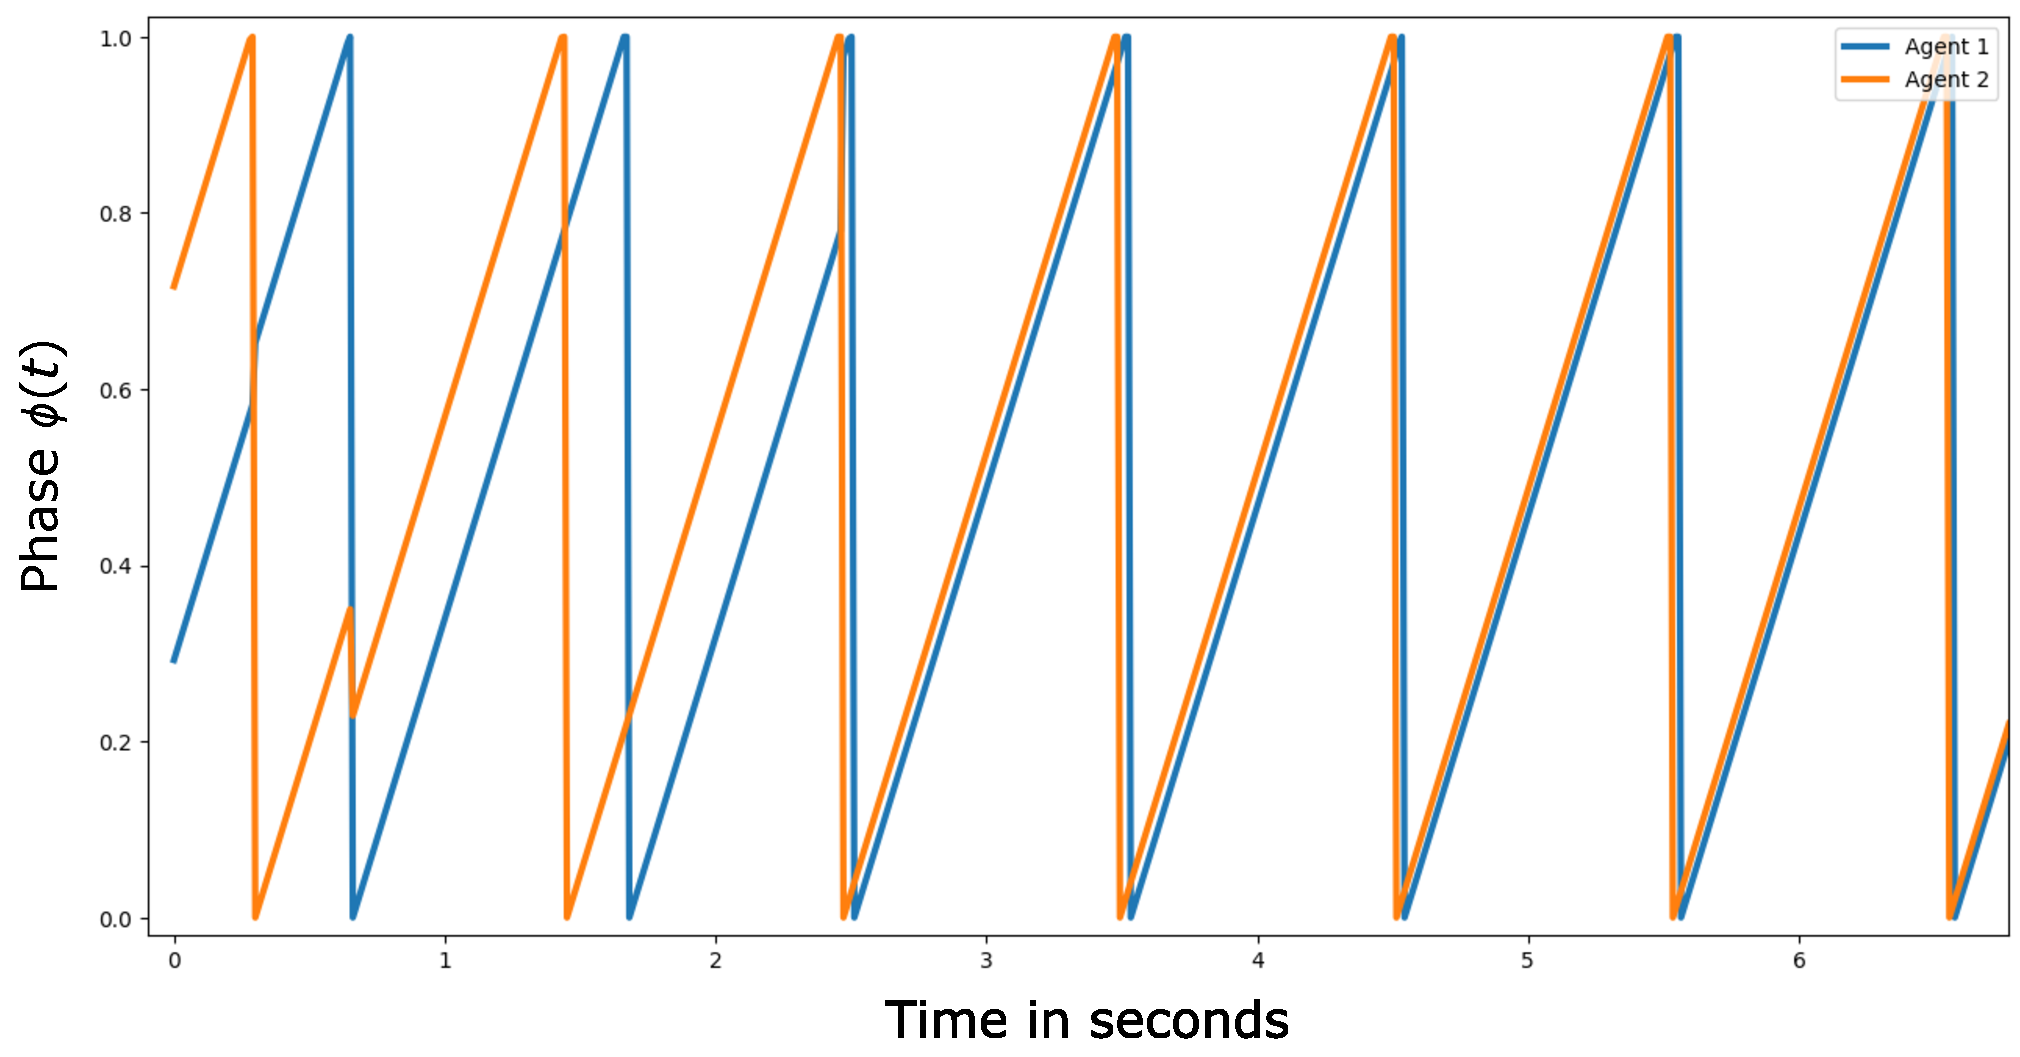
\includegraphics[width=0.9\linewidth]{Assets/Figures/KNymoenPhaseAdjustmentSecondTry.pdf}
		\caption[Illustration of K. Nymoen's bi-directional phase-adjustment]{Bi-directional phase-adjustment with K. Nymoen et al.'s approach}
		\label{fig:nymoen_phase}
	\end{figure}
	
	
	

	% PHASE.-ADJ APPROACH 3: HIGH LEVEL Self-Awareness
	% Hopefully an improved method with some additional Self-Awareness components
	\subsection{Thorvaldsen's self-aware phase-adjustment}
	
	\gjor{Beskriv min nye proposede algoritme (to-be-implemented) for å oppnå harmonisk synkronitet i $\phi$-problemet med phase-adjustment, som inneholder flere tilleggs- Self-Awareness-komponenter, sammenliknet med K. Nymoens bi-directional phase-adjustment metode. 
	
	Eksempler på slike tilleggs- Self-Awareness-komponenter er såkalt Belief-awareness (som fanger usikkerhet og tillits-nivåer) og/eller Expectation-awareness (som kombinerer Belief-awareness og Time-awareness) \cite{sacs17_ch3}. Andre forslag er å implementere Self-Awareness i forhold til:
	\begin{itemize}
		\item avstand: f.eks. $H^*(n)= H(n) \cdot \frac{1}{distance}$ for ``fire''-event $n$, så lenge ikke $distance = 0$.
		\item hvem som er hvem (i.e. agent\_id).
		% \item de andres frekvenser. Høre etter og registrere andre individers ``fire''-signaler kontinuerlig og estimere disse individenes frekvenser utifra det (f.eks. $\hat{\omega}_j = time_{j, fired\_now} - time_{j, fired\_last\_time}$, eller et gjennomsnitt av slike oppsamlede verdier).
	\end{itemize}
	}
	
	
	
	










	

% SECTION 3, Presenting new Methods I implemented myself for Frequency-Synchronization:
\section{Synchronizing oscillator-frequencies}
\label{sec:frequency_methods}

	\gjor{Introduser det andre, og mer utfordrende, $\phi$-\&$\omega$-problemet, uthevet og i fet skrift. Deretter løsningene dens (Freq.-Adj.-metodene), som man må bruke i tillegg til $\phi$-løsningene eller Phase-Adjustment-metodene. "This is the second and harder problem of synchronizing both phases $\phi_i$, as well as frequencies $\omega_i$, for all agents $i$."}

	% Om Update-functions for frekvens-oppdateringene
	When we open up for the possibility for heterogenous frequencies in our musical agent collective, we open up to exciting musical aspects like the playing of diverse rhythmic patterns as e.g. mentioned in Section \ref{sec:harmonic_synchrony}, but we then also need to not only synchronize phases, but also frequencies, simultaneously. This second problem of adjusting synchronizing both all phases $\phi_i$ and frequencies $\omega_i$, the values of which can all be heterogenous and initially random, for all agents $i$ in the agent collective — we will from here on and out refer to as \textbf{the $\phi$-\&$\omega$-problem}. This slightly more complex problem calls for us to also find solutions on how to adjust and synchronize frequencies. We already have methods by which we can adjust and synchronize the agents's phases $\phi$ with, described in Section \ref{sec:phase_methods}, but we do so-far lack methods by which we can adjust and synchronize the agents's frequencies $\omega$ with.
	
	We hence now introduce randomly initialized, non-constant, and heterogenous oscillator-frequencies in our musical agents. The agents are now required to synchronize their initially different and random frequencies, so that frequencies are ``legal'' and \textit{harmonically synchronized}. Such ``legal'' frequencies are described clearly in detail in Section \ref{sec:harmonic_synchrony}.
	
	Some implemented approaches for achieving this are presented now. Notice the increasing degree of \textit{Computational Self-Awareness} endowed in the methods.
	
	
	% FREQ.-SYNCH APPROACH 2: MID LEVEL Self-Awareness
	% K. Nymoen's Frequency-Synchronization with some Self-Awareness
	\subsection{K. Nymoen's middle SA-leveled frequency-adjustment}
	
	In the newly proposed Unity simulator environment, the previously introduced self-assessed synch-score $s(n)$ (in \ref{s_n}) is implemented as a list containing \textit{m} error-scores $\epsilon$. Such a list is easily implemented in C\# by declaring a List$<$float$>$ called \textit{errorBuffer} e.g. (i.e. \textit{errorBuffer} is a list containing floating point values):
	
	\begin{equation}
	\label{error_buffer}
		errorBuffer = \{\epsilon(n), \epsilon(n-1), ... , \epsilon(n-m)\},
	\end{equation} \nl
	
	then leading to:
	
	\begin{equation}
	\label{self_assessed_synch}
		\begin{array}{rrclcl}
		s(n) & = & median(errorBuffer) \\ 
		& = & median(\{\epsilon(n), \epsilon(n-1), ... , \epsilon(n-m)\}) \in [0, 1],
		\end{array}
	\end{equation} \nl
	
	where $n$ is the latest observed ``fire-event'', and $m$ is the number of the last observed ``fire''-events we would like to take into account when calculating the self-assessed synch-score. \nl
	
	Regarding the ``frequency-update-contributions'' (the $H$-values described in \ref{H_n}) in my Unity-simulator, all the calculated H-values are accumulated and stored in an initially empty C\#-list (of floats), referred to as $H(n)$, at once they are calculated. The $H(n)$-list is then consecutively ``cleared out'' or ``flushed'' when its H-values have been used for the current cycle/period's frequency adjustment (i.e. at the phase climax, when $\phi(t)=1$), and is then ready to accumulate new H-values during the next cycle/period.
	
	
	% FREQ.-SYNCH APPROACH 3: HIGH LEVEL Self-Awareness
	% Hopefully an improved method with some additional Self-Awareness components
	\subsection{Thorvaldsen's high SA-leveled frequency-adjustment}
	
	\gjor{Beskriv min nye proposede algoritme (to-be-implemented) for å oppnå harmonisk synkronitet i $\phi$- \& $\omega$-problemet med frequency-adjustment, som inneholder flere tilleggs- Self-Awareness-komponenter, sammenliknet med K. Nymoens frequency-adjustment metode. Eksempler på slike tilleggs- Self-Awareness-komponenter er såkalt Belief-awareness (som fanger usikkerhet og tillits-nivåer) og/eller Expectation-awareness (som kombinerer Belief-awareness og Time-awareness) \cite{sacs17_ch3}. Andre forslag er å implementere Self-Awareness i forhold til, og vekte frekvensoppdaterings-bidragene H(n) i henhold til:
	\begin{itemize}
		\item avstand: f.eks. $H^*(n)= H(n) \cdot \frac{1}{distance}$ for ``fire''-event $n$, så lenge ikke $distance = 0$.
		\item hvem som er hvem (i.e. agent\_id).
		\item større median-liste ift. den self-assessed'e synch-score'n $s(n)$ og $errorBuffer$'et. Dette kan være nyttig ved større collective-sizes, da et lite/kort median-filter/-$errorBuffer$-liste vil kunne miste eller gå glipp av error-scores, $\epsilon(n)$, fra ``fire''-events fra langt tilbake (tidlig) i ``oppsamlings-perioden.''
		\item de andres frekvenser. Høre etter og registrere andre individers ``fire''-signaler kontinuerlig og estimere disse individenes frekvenser utifra det (f.eks. $\hat{\omega}_j = time_{j, fired\_now} - time_{j, fired\_last\_time}$, eller et gjennomsnitt av slike oppsamlede verdier).
	\end{itemize}
	}






% SECTION 4, Om target-staten til systemet: harmonic synchrony
\section{System target state: harmonic synchrony}
\label{sec:harmonic_synchrony}

As previously mentioned, this state of \textit{harmonic synchrony} is then the system goal state which we want the musical robot-collective to end up in eventually, and the sooner the better.

The state of harmonic synchrony is defined as the state in which all agents in the musical collective ``fire''/``flash'', as described in Subsection \ref{subsec:fire_signal}, at an even and underlying interval or pulse, a certain number of times in a row. This is not to say all agents will have to ``fire''/``flash'' simultaneously, as has traditionally been the case for pulse-coupled oscillators \cite{}. So in a way, for phases $\phi$ to be harmonically synchronized, all agent ``fire''-signals will have to coincide in a way, even though they don't all have to incur exactly at the same time always. Exactly how this can look is (to-be) shown in Section \ref{sec:performance_measure}.

As one is designing and creating an interactive music technology system, one might want to encourage and allow for the playing of various musical instruments at various rhythms/paces, as it might be quite boring if all instruments were played at the exact same measure or pulse. As K. Nymoen et al. \cite{nymoen_synch} reason when discussing their own interactive ``Firefly'' music-system, as well as coining the term of harmonic synchrony: \nl

\textit{Temporal components in music tend to appear in an integer-ratio relation to each other (e.g., beats, measures, phrases, or quarter notes, 8ths, 16ths)}. \nl

and \nl

\textit{Being an interactive music system, people may want their device to synchronize with different subdivisions of a measure (e.g. some play quarter notes while others play 8ths).} \nl

Accomodating for these aspects then, K. Nymoen et al. took inspiration for achieving synchronization in a decentralized system from the concept of \textit{harmonics} in the frequency spectrum of a waveform, in that each harmonic wave or overtone has a frequency with an integer-relationship to the fundamental (smallest) frequency. This phenomenon can e.g. be seen in the frequency spectrogram of a humanly hummed G3-tone, depicted in Figure \ref{fig:sub:G3_hummed_waveform}, where one can observe the presence of harmonics and overtones having frequencies with integer relationships to the fundamental (smallest) frequency which was intended to be at 195,99 Hz.

\begin{figure}[ht!]
	\centering
		\begin{subfigure}[t]{.5\textwidth}
			\centering\captionsetup{width=.9\linewidth}%
			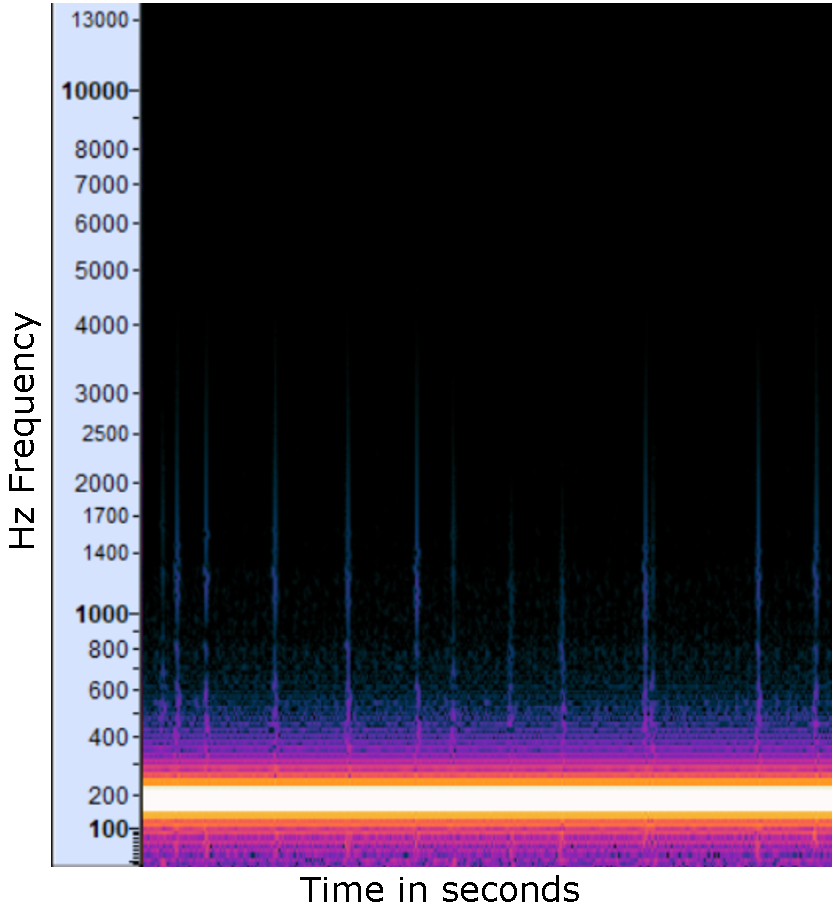
\includegraphics[width=0.9\linewidth]{Assets/Figures/G3_196Hz_PureTone_waveform_spectrogram.pdf}
			\caption{The frequency spectrogram of the audible waveform being a monotone and purely generated G3-tone at 195,99 Hz \cite{generate_tones}.}
			\label{fig:sub:G3_pure_waveform}
		\end{subfigure}%
		\begin{subfigure}[t]{.5\textwidth}
			\centering\captionsetup{width=.9\linewidth}%
			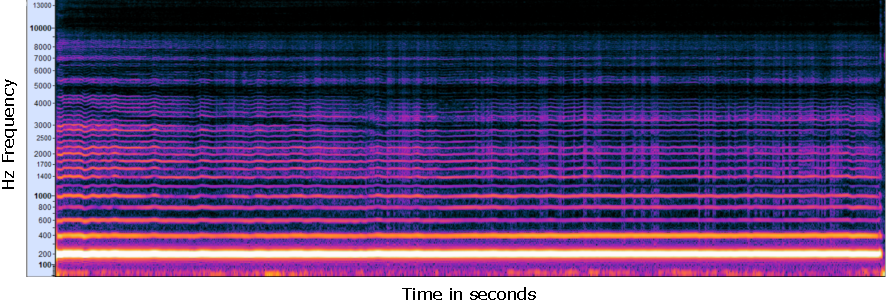
\includegraphics[width=0.9\linewidth]{Assets/Figures/G3_196Hz_HummingWaveform_FrequencySpectrum.pdf}
			\caption{The frequency spectrogram of the audible waveform being a more-or-less monotone but non-pure G3-tone, hummed and recorded by me \cite{}, as I tried to repeat the tone in \ref{fig:sub:G3_pure_waveform} with my voice.}
			\label{fig:sub:G3_hummed_waveform}
		\end{subfigure}
	\caption[Frequency spectrograms illustrating the absence and presence of harmonics and overtones in audible waveforms]{Frequency spectrograms of two different-sounding waveforms of the same G3-tone at 195,99 Hz. Note the absence and presence of harmonics and overtones in waveform \ref{fig:sub:G3_pure_waveform} and \ref{fig:sub:G3_hummed_waveform} respectively. Frequencies in a harmonically synchronized agent collective will for the first $\phi$-problem resemble the frequencies in \ref{fig:sub:G3_pure_waveform}, where all frequencies are equal and constant. Conversely, when frequencies can be heterogenous and unequal, as in the $\phi$- \& $\omega$-problem, the frequencies in a harmonically synchronized agent collective will rather resemble the frequencies in \ref{fig:sub:G3_hummed_waveform}, where these higher frequencies with integer-relationships to the fundamental and lowest frequency can be present.}
	\label{fig:frequency_spectrograms}
\end{figure}

More accurately then, and inspired by although not completely analagous to the integer-relationship frequencies like in Figure \ref{fig:sub:G3_hummed_waveform}, we introduce the formal and ``legal'' requirement the oscillator-frequencies in the musical robot collective have to fulfill in order for the oscillator-frequencies to be harmonically synchronized. All musical agents—in a harmonically synchronized state—will have frequencies $\in \omega_{0} \cdot 2^{\mathbb{N}_0}$, where $\omega_{0}$ is the agent with the lowest frequency's frequency (i.e. the fundamental frequency), and $\mathbb{N}_0$ is the mathematical set of natural numbers including the number zero. Hence, agents will typically have frequencies like $\omega_{0} \cdot 2^0 = \omega_{0}$, $\omega_{0} \cdot 2^1 = 2\omega_{0}$, $\omega_{0} \cdot 2^2 = 4\omega_{0}$, or $\omega_{0} \cdot 2^3 = 8\omega_{0}$. If all agents end up with these kind of frequencies, we say they have ``legal'' and harmonically synchronized frequencies.







% SECTION 5, Presenting the Performance-measure used to evaluate the implemented methods:
\section{Performance-measure: time until system target state of harmonic synchrony is detected}
\label{sec:performance_measure}

The performance-measure we will use to evaluate our implemented methods with, is the time it takes for the agent collective to achieve the system target state of harmonic synchrony, also referred from here on and out as HSYNCHTIME. The question then becomes: how does one detect harmonic synchrony in an musical agent collective?

In order for the collective to be considered harmonically synchronized, a set of conditions have to be met:

\begin{itemize}
	\item Firings may only happen within a short time period $t_f$.
	\item Between each $t_f$, a period $t_q$ without fire events must be equally long $k$ times in a row.
	\item All nodes must have fired at least once during the evaluation period.
\end{itemize}

E.g., as K. Nymoen et al. did, one could have the short time-period during which agents are allowed to fire, $t_f$, be equal to say 80ms, and $k=8$. $t_q$ is not defined, as it depends on the frequency to which the nodes converge.

$t_q$ is also then reset when a firing is observed within the ``illegal'' $t_q$-window.

When all the conditions above have been met, we have detected harmonic synchrony, and we also then have our synchrony-/performance-score, being the time from the start of the simulation until now, HSYNCHTIME.

An illustration of such a detection of harmonic synchrony is given below in Figure \ref{fig:node_firing_plot}.

\begin{figure}[h]
	\centering
	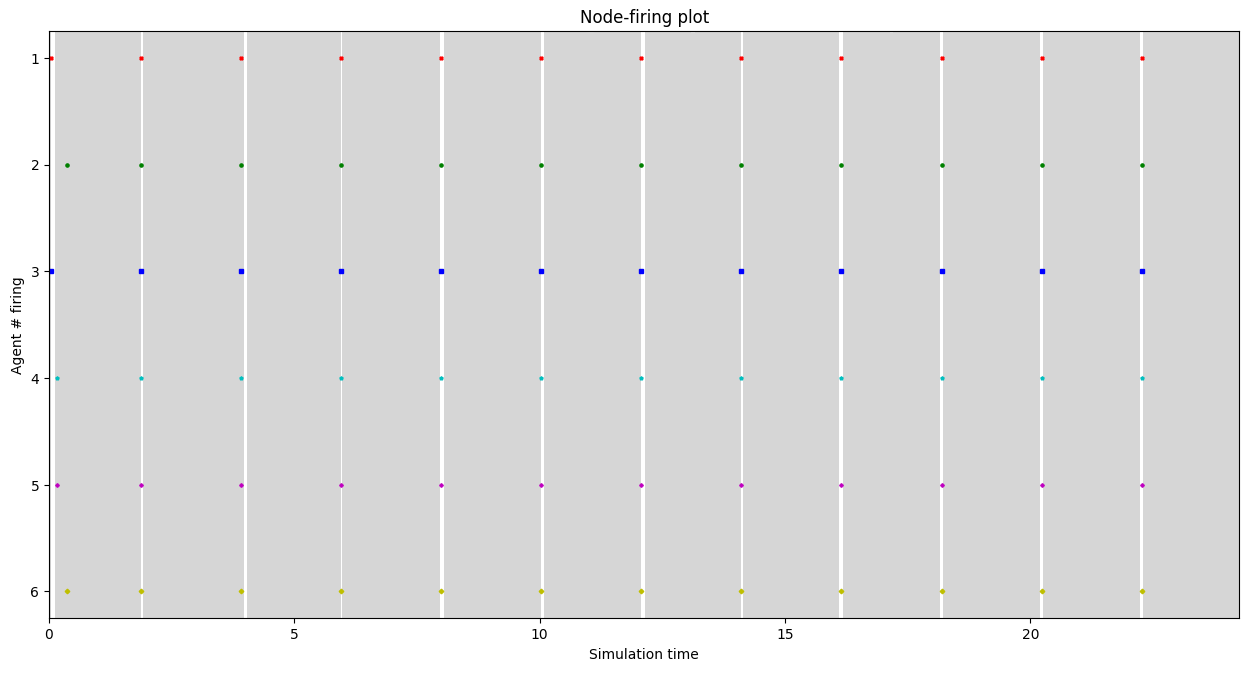
\includegraphics[width=\linewidth]{Assets/Figures/aNicerNodeFiringPlotOfASuccessfulSynchronizationButWithWeirdTimewindows.png}
	\caption[A node-firing (performance-)plot, demonstrating how the system target state of harmonic synchrony is detected]{A node-firing plot, demonstrating how the system target state of harmonic synchrony is detected eventually.}
	\label{fig:node_firing_plot}
\end{figure}
	
	% EXPERIMENTS AND RESULTS
	\chapter{Experiments and Results}
	\besk{Skal følge opp \textit{research questions}'a mine ved en diskusjon av til hvilken grad og på hvilke måter arbeidet har besvart dem}

	\gjor{Vurder å dele opp som Tønnes: Først 1) Evolusjonære/\opphoy{Simulator} eksperimenter og resultater, så 2) Fysiske eksperiment og resultater}
	
	\gjor{Legg inn performance-plot av initielt Simulator-eksperiment for synkroniseringstider for f.eks. Mirollo-Strogatz vs. Nymoen et al.'s fase-justering}
	
	% DISCUSSION
	\section*{Discussion}
	% SE PÅ TØNNES SIN MASTEROPPGAVE FOR INSPIRASJON.



% FOOTER
	% BIBLIOGRAPHY
	\newpage
	\printbibliography
	
	% APPENDICES (A, B, C, D, ...)
	% APPENDIX A HERE
	% APPENDIX B HERE
\end{document}